\documentclass{article}
\usepackage[a4paper]{geometry}
\newgeometry{margin=0pt}
\pagestyle{empty}
\usepackage{style}
\usepackage{graphicx}
\usepackage{ragged2e}
\usepackage{hyperref}
\usepackage{tikz}
\tikzstyle{dot}=[circle,fill,inner sep=2pt]

\makeatletter
\newcommand{\rubric}[1]{
    \centering
    \vspace{1cm}
    \section*{#1}
    \hrule
    \vspace{0.3cm}
    \raggedright
}

\begin{document}

\noindent\colorbox{black}{
    \begin{minipage}[t][0.98\textheight][t]{0.33\textwidth}
        \centering  \color{white} \bfseries
        \vspace{1cm}
        \includegraphics[width=0.8\textwidth]{arnaud-cv}
        \vspace{0.5cm}

        \Huge \texttt{Arnaud Pannatier} \\
        \vspace{0.4cm}
        \normalsize  { \color{dimmedwhite} SOFTWARE ENGINEER } \\
        \vspace{1.4cm}
        \Large \texttt{PROFILE} \\

        \small \color{dimmedwhite} \justifying
        \vspace{0.4cm}
        \begin{quotation}
            \color{dimmedwhite}
            \noindent I am a Ph.D. Student in François Fleuret's Machine Learning group (Idiap/EPFL). My main research interest are deep learning architectures and their applications on High-Altitude Wind Nowcasting.
        \end{quotation}

        \vfill
        \begin{quotation}
            \noindent
            \href{mailto:arnaud.pannatier@idiap.ch}{arnaud.pannatier@idiap.ch}\\
            \href{https://arnaudpannatier.ch}{https://arnaudpannatier.ch}\\
            \\
            \noindent
            Rue des Longs-Prés 40 \\
            3960 Sierre \\
            VS, Switzerland \\
            \\
            \noindent Born 20 September 1995 \\
            Married, one child (2022) \\

        \end{quotation}
        \vspace{1cm}

    \end{minipage}
}
\hspace{0.05\textwidth}
\begin{minipage}[t][0.98\textheight][t]{0.5\textwidth}
    \rubric{Education}

    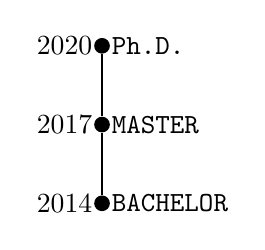
\begin{tikzpicture}
        \node[dot] (2020) at (0,2) {};
        \node[dot] (2017) at (0,1) {};
        \node[dot] (2014) at (0,0) {};
        \draw (2020)node[left] {2020};
        \draw (2020)node[right] {\texttt{Ph.D.}};
        \draw (2017)node[left] {2017};
        \draw (2017)node[right] {\texttt{MASTER}};
        \draw (2014)node[left] {2014};
        \draw (2014)node[right] {\texttt{BACHELOR}};
        \draw (2014) -- (2017) -- (2020);
    \end{tikzpicture}


    \rubric{Publications}

    Test test

    \rubric{Skills}

    \rubric{Languages}

    \rubric{Hobbies \& Interest}

\end{minipage}


\end{document}